\section{直线相关的题型}

\subsection{直线过定点问题}

\begin{theorem}
    直线恒过顶点，是让参数的影响消失。若直线方程含参数 $m$ ，将其化成：
    $m \square+\Delta=0$ 的形式，其中 $\square$ 和 $\triangle$ 是不含 $m$ 的式子。

    则方程组 $\left\{\begin{array}{l}\square=0 \\ \Delta=0\end{array}\right.$ 的解就是直线所过定点。
\end{theorem}

\begin{example}
    \begin{itemize}
        \item 求直线 $(m+1)x+my-2m-1=0$ 恒过的定点。
        \item 求直线 $y=kx+2k$ 过的定点。
    \end{itemize}
\end{example}

\v{4em}

\begin{example}
    求直线所过的定点。
    \begin{itemize}
        \item 不论 $m$ 取何值，直线 $2 m x+(m+1)(x-y)+y-5=0$ 恒过定点。
        \item （2）直线 $(2 m+1) x+(m+1) y=7 m+4$ 恒过定点。
    \end{itemize}
\end{example}

\v{4em}

\begin{example}
    求证：直线 $\left(2 m^2+8 m+3\right) x-\left(3 m^2+m-4\right) y+4 m^2-6 m-11=0$ ，无论m取何值，该直线恒过定点．
\end{example}

\v{4em}

\begin{example}
    已知函数 $f(x)=\mathrm{e}^x+a x+1$ ．
    若函数 $f(x)$ 的图象恒过定点 $P$ ，且在定点 $P$ 处的切线方程与直线 $3 x+y+1=0$ 平行，求定点 $P$ 的坐标和实数 $a$ 的值；
\end{example}

\v{6em}

\begin{example}
    对任意的实数 $k$ ，直线 $y=k x+1$ 与圆 $x^2+y^2=2$ 的位置关系是（\qquad）
    \begin{tasks}(4)
        \task 相离
        \task 相切
        \task 相交但直线不过圆心
        \task 相交且直线过园心
    \end{tasks}
\end{example}

\v{6em}

\begin{example}
    已知直线 $l_1: x+(m+1) y+1=0, l_2:(m+1) x+y-1=0$ ．
    \begin{itemize}
        \item 若 $l_1 / / l_2$ ，求 $m$ 的值．
        \item 设直线 $l_1$ 过的定点为 $A$ ，直线 $l_2$ 过的定点 $B$ ，且当 $m=1$ 时，直线 $l_1$ 与 $l_2$ 交点为 $C$ ，求 $\triangle A B C$ 中 $B C$ 边上的高所在直线的方程．
    \end{itemize}
\end{example}

\v{6em}

\begin{example}
    若关于 $t$ 的方程 $(t^2-1)x+ty+t=0$ 表示过定点的一簇直线，求该定点的坐标。
\end{example}

\begin{solution}
    设定点坐标为 $(x_0,y_0)$，则对任意 $t$，有：
    \[
        (t^2-1)x_0+ty_0+t=0
    \]

    将上式展开并按 $t$ 的幂次整理：
    \[
        t^2x_0+t(y_0+1)-x_0=0
    \]

    由于该等式对任意 $t$ 成立，所以 $t$ 的各次幂系数必须为零：
    \[
        \begin{cases}
            x_0=0   \\
            y_0+1=0 \\
            -x_0=0
        \end{cases}
    \]

    所以定点坐标为 $(0,-1)$。
\end{solution}

\subsection{直线和线段有交点}

\begin{theorem}
    可以直接求端点的斜率出来，也可以用线性规划的知识来解决。
\end{theorem}

\begin{example}
    已知直线 $k x-y+2=0$ 和以 $M(3,-2), ~ N(2,5)$ 为端点的线段相交，则实数 $k$ 的取值范围为 （\qquad）
    \begin{tasks}(4)
        \task $\left(-\infty,-\frac{4}{3}\right]$
            \task $\left[\frac{3}{2},+\infty\right)$
        \task $\left[-\frac{4}{3}, \frac{3}{2}\right]$
        \task $\left(-\infty, \frac{4}{3}\right] \cup\left[\frac{3}{2},+\infty\right)$
    \end{tasks}
\end{example}

\vspace{6em}

\begin{example}
    已知点 $A(-2,3), ~ B(3,-1)$ ，若直线 $l$ 过点 $P(0,-1)$ 且与线段 $A B$ 相交，则直线 $l$ 的斜率 $k$ 的取值范围是 \underline{\qquad}
\end{example}

\vspace{4em}

\subsection{点到直线的距离公式}

\begin{theorem}[点到直线的距离公式]
    点 $P(x_0, y_0)$ 到直线 $Ax + By + C = 0$ 的距离 $d$ 为
    \[
        d = \frac{|Ax_0 + By_0 + C|}{\sqrt{A^2 + B^2}}.
    \]
    其中 $A, B$ 不同时为 $0$，且 $A^2 + B^2 \neq 0$.
\end{theorem}

\begin{example}
    求点 $P(3,4)$ 到直线 $2x - y + 5 = 0$ 的距离。
\end{example}

\begin{solution}
    将 $P(3,4)$ 和直线 $2x - y + 5 = 0$ 的系数代入，得：
    \[
        d = \frac{|2 \cdot 3 - 1 \cdot 4 + 5|}{\sqrt{2^2 + (-1)^2}} = \frac{|6 - 4 + 5|}{\sqrt{5}} = \frac{7}{\sqrt{5}} = \frac{7\sqrt{5}}{5}
    \]
\end{solution}

\begin{example}
    求点 $P(2,-1)$ 到直线 $x - 2y + 3 = 0$ 的距离，并求点 $P$ 在该直线上的投影点坐标。
\end{example}

\v{4em}

\subsection{两直线方程组的解关系}

\begin{example}
    直线 $l_1: A_1 x+B_1 y+C_1=0$ 和直线 $l_2: A_2 x+B_2 y+C_2=0$ 的位置关系如表所示：

    \begin{center}
        \begin{tabular}{|l|l|l|l|}
            \hline 方程组 $\left\{\begin{array}{l}A_1 x+B_1 y+C_1=0, \\ A_2 x+B_2 y+C_2=0\end{array}\right.$ 的解 & 一组                   & 无数组   & 无解                   \\
            \hline 直线 $l_1$ 与 $l_2$ 的公共点个数                                                                   & 1                    & \quad & 零个                   \\
            \hline 直线 $l_1$ 与 $l_2$ 的位置关系                                                                    & $\underline{\qquad}$ & 重合    & $\underline{\qquad}$ \\
            \hline
        \end{tabular}
    \end{center}
\end{example}

\pagebreak

\begin{problemset}
    \item 过点 $(-2,0)$ 与圆 $x^2+y^2-6 x=0$ 相切的两条直线的夹角为 $\alpha$ ，则 $\sin \alpha=$ \underline{$\qquad$} ．
    \item 两直线 $y=x-1$ 与 $x-2 y+1=0$ 的夹角为 \underline{$\qquad$} ．（结果用反三角表示）
    \item 已知直线过点 $P(2,2)$ 且倾斜角为 $135^{\circ}$ ，则点 $Q(-2,0)$ 到直线 $l$ 的距离为 \underline{$\qquad$} ．
    \item 已知直线 $l$：$(m+1) x+(2 m-1) y+m-2=0$ ，则直线恒过定点 \underline{\qquad}.
    \item 直线 $(m-1) x+(m-3) y-2=0$ 与圆 $(x-1)^2+y^2=1$ 的位置关系是 \underline{\qquad}
    \item 图中曲线为圆或半圆，已知点 $P(x, y)$ 是阴影部分（包括边界）的动点，则 $\frac{y}{x-4}$ 的最小值为 \underline{\qquad}
    \begin{figure} [H]
        \centering
        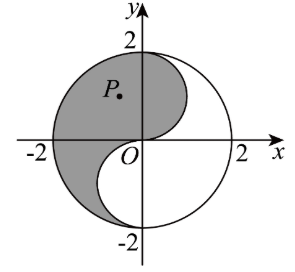
\includegraphics[width=0.2\textwidth]{chapters/linear-circle/images/直线相关的题型/img-20250713004105.png}
    \end{figure}
    \item 已知圆 $C$ 的方程为 $x^2+y^2-2 y-1=0, ~ P(a, b)$ 为圆 $C$ 上任意一点，则 $\frac{2 a+b-5}{a-2}$ 的取值范围为 （\qquad）
    \begin{tasks}(4)
        \task $[-1,2]$
        \task $(-\infty,-1] \cup[2,+\infty)$
                    \task $[1,3]$
                    \task $(-\infty, 1] \cup[3,+\infty)$
    \end{tasks}
\end{problemset}

\subsection{练习答案}
\begin{tips}
    \begin{enumerate}
        \item 过点 $(-2,0)$ 与圆 $x^2+y^2-6 x=0$ 相切的两条直线的夹角为 $\alpha$ ，则 $\sin \alpha= \frac{24}{25}$ ．
        \item 两直线 $y=x-1$ 与 $x-2 y+1=0$ 的夹角为 $arctan\frac{1}{3}$
        \item 已知直线过点 $P(2,2)$ 且倾斜角为 $135^{\circ}$ ，则点 $Q(-2,0)$ 到直线 $l$ 的距离为 $3\sqrt{2}$ ．
        \item 已知直线 $l$：$(m+1) x+(2 m-1) y+m-2=0$ ，则直线恒过定点 \underline{$(1,-1)$}.
        \item 直线 $(m-1) x+(m-3) y-2=0$ 与圆 $(x-1)^2+y^2=1$ 的位置关系是 \underline{相交或相切（点在圆上）}
        \item 图中曲线为圆或半圆，已知点 $P(x, y)$ 是阴影部分（包括边界）的动点，则 $\frac{y}{x-4}$ 的最小值为 $-\frac{8}{15}$.
        \item 提示：将 $\frac{2 a+b-5}{a-2}=\frac{2(a-2)+b-1}{a-2}=2+\frac{b-1}{a-2}$
    \end{enumerate}
\end{tips}

\v{6em}

\subsection{点关于直线对称}

\begin{theorem}[点关于直线的对称]
    若两点 $A(x_1, y_1), B(x_2, y_2)$ 关于直线 $ax+by+c=0$ 对称，则线段 $AB$ 的中点在直线上，且直线 $AB$ 与该直线垂直。
\end{theorem}

\begin{example}
    \begin{itemize}
        \item[(1)] 已知点 $A(2,3)$ 关于直线 $l: 3x+4y-10=0$ 的对称点为 $B$. 求点 $B$ 的坐标.

        \item[(2)] 已知点 $P(1,2)$ 关于某直线 $l$ 对称得到点 $Q(-3,4)$. 求直线 $l$ 的方程.
    \end{itemize}
\end{example}

\v{6em}

\begin{example}
    线段的垂直平分线问题：
    \begin{itemize}
        \item[（1）] 已知两点 $A(7,-4), ~ B(-5,6)$ 求线段 $A B$ 的垂直平分线的方程．
        \item[（2）] 求经过两条直线 $2 x+y-8=0$ 和 $x-2 y+1=0$ 的交点，且平行于直线 $4 x-3 y-7=0$ 的方程．
    \end{itemize}
\end{example}

\vspace{4em}

\subsection{直线关于直线对称}

\begin{theorem}
    转化为点到直线的对称问题即可。
\end{theorem}

\begin{example}
    已知直线 $l_1: 2x-y+3=0$ 关于直线 $l_2: x+2y-4=0$ 对称，得到直线 $l_3$。求直线 $l_3$ 的方程。
\end{example}

\v{4em}

\subsection{点到直线的最大距离}

\begin{theorem}
    点到直线的最大距离等于点到直线的垂直距离。
\end{theorem}

\begin{example}
    已知点 $A(-1,0)$ 和点 $B$ 关于直线 $l: x+y-1=0$ 对称。

    若直线 $l_1$ 过点 $B$ ，且使得点 $A$ 到直线 $l_1$ 的距离最大，求直线 $l_1$ 的方程．
\end{example}

\vspace{4em}

\subsection{斜率构造}

\begin{theorem}
    形如 $\frac{y-k}{x-h}$ 的式子可以构造为平面上一点 $(x,y)$ 与点 $(h,k)$ 形成的斜率。
\end{theorem}

\begin{example}
    在平面直角坐标系 $x O y$ 中，动点 $M(x, y)$ 到 $A(-1,0) 、 B(1,0)$ 两点的距离的平方和为 $10$ ，则 $\frac{y+2}{x-1}$ 的取值范围为 \underline{\qquad}
\end{example}

\v{6em}

\begin{example}
    已知坐标平面内三点 $A(-2,-4), B(2,0), C(-1,1)$ ．
    \begin{itemize}
        \item[(1)] 若 $A, B, C, D$ 可以构成平行四边形，且点 $D$ 在第一象限，求点 $D$ 的坐标；
        \item[(2)] 若 $E(m, n)$ 是线段 $A C$ 上一动点，求 $\frac{n}{m-2}$ 的取值范围．
    \end{itemize}
\end{example}

\v{6em}

\subsection{直线与坐标轴形成的三角形}

\begin{theorem}
    直线与坐标轴形成的三角形面积等于 $\frac{1}{2}$ 乘以直线与 $x$ 轴、$y$ 轴的截距的绝对值之积。
\end{theorem}

\begin{example}
    已知直线 $l: 2 x+3 y-6=0$ 与坐标轴围成的三角形面积为 \underline{\qquad}
\end{example}

\v{6em}

\begin{example}
    已知直线 $l_1$ 的方程为 $y=-2 x+3$ ．
    \begin{enumerate}
        \item 若直线 $l_2$ 与 $l_1$ 平行，且过点 $(-1,3)$ ，求直线 $l_2$ 的方程；

        \item 若直线 $l_2$ 与 $l_1$ 垂直，且 $l_2$ 与两坐标轴围成的三角形面积为 4 ，求直线 $l_2$ 的方程
    \end{enumerate}
\end{example}

\v{4em}

\subsection{直线与最值问题}

\begin{example}
    求过 $(1,2)$ 的直线和 $X$ 轴、$Y$ 轴正半轴形成的三角形的面积最小值。
\end{example}

\v{6em}

\begin{example}
    如图，某房地产公司要在荒地 ABCDE 上划出一块长方形土地（不改变方向）建造一幢 8 层的公寓，如何设计才能使公寓占地面积最大？
\end{example}

\begin{tikzpicture}[
        % 定义单位，减小比例
        x=0.06cm, % 从0.1cm缩小到0.06cm
        y=0.06cm, % 从0.1cm缩小到0.06cm
        % 轴线样式
        axis/.style={->, >=Stealth, thick},
        % 点的样式
        point/.style={circle, fill, inner sep=1pt},
        % 标签样式
        label_style/.style={font=\scriptsize},
        dim_label/.style={font=\tiny, fill=white, inner sep=0.5pt} % 尺寸标注的背景为白色
    ]

    % 绘制坐标轴
    \draw[axis] (0,0) -- (120,0) node[right, label_style] {$x$};
    \draw[axis] (0,0) -- (0,95) node[above, label_style] {$y$};

    % 标注原点O
    \node[label_style, below left=1pt] at (0,0) {$O$};

    % 定义关键点坐标
    \coordinate (O) at (0,0);
    \coordinate (A) at (0,20); % 80 - 60 = 20
    \coordinate (B) at (30,0); % 100 - 70 = 30
    \coordinate (C) at (100,0);
    \coordinate (D) at (100,80);
    \coordinate (E) at (0,80);

    % 绘制矩形 CDEO (或者说整个大区域)
    \draw (O) -- (C) -- (D) -- (E) -- cycle; % O-C-D-E-O

    % 绘制线段 AB
    \draw[thick] (A) -- (B);

    % 绘制点 P
    \coordinate (P) at (0.3*30, 0.7*20); % P大约在线段AB的中间偏A一点
    \node[point] at (P) {};
    \node[label_style, below left=1pt] at (P) {$P$}; % 标注点P

    % 标注图中的点 A, B, C, D, E
    \node[label_style, above left=1pt] at (A) {$A$};
    \node[label_style, below right=1pt] at (B) {$B$};
    \node[label_style, below right=1pt] at (C) {$C$};
    \node[label_style, above right=1pt] at (D) {$D$};
    \node[label_style, above left=1pt] at (E) {$E$};

    % 标注尺寸
    % 水平尺寸
    \draw[<->] (0,85) -- (100,85) node[midway, above, dim_label] {$100 \text{ m}$};
    \draw[<->] (30,-5) -- (100,-5) node[midway, below, dim_label] {$70 \text{ m}$};

    % 垂直尺寸
    \draw[<->] (-5,0) -- (-5,80) node[midway, left, dim_label] {$80 \text{ m}$};
    \draw[<->] (-5,20) -- (-5,80) node[midway, left, dim_label] {$60 \text{ m}$};

    % 绘制图中虚线部分
    \draw[dashed] (0,20) -- (100,20); % 从A点向右的虚线
    \draw[dashed] (30,0) -- (30,80); % 从B点向上的虚线
\end{tikzpicture}

\subsection{直线和对称光学}

\begin{example}
    光线从点 $A(2,3)$ 射出，若镜面的位置在直线 $l: x+y+1=0$ 上，反射光线经过 $B$ $(1,1)$ ，求入射光线和反射光线所在直线的方程，并求光线从 $A$ 到 $B$ 所走过的路线长．
\end{example}

\begin{tips}
    求出点 $\boldsymbol{A}$ 关于 $\boldsymbol{l}$ 的对称点，就可以求出反射光线的方程，进一步求得入射点的坐标，从而可求入射光线方程，可求光线从 $\boldsymbol{A}$ 到 $\boldsymbol{B}$ 所走过的路线长．
\end{tips}

\v{6em}

\subsection{直线方程的综合辨析}

\begin{example}
    下列四个选项中，说法错误的是（\hspace{2em}）
    \begin{itemize}
        \item  坐标平面内的任何一条直线均有倾斜角和斜率
        \item  直线 $a x+2 y+6=0$ 与直线 $x+(a-1) y+a^2-1=0$ 互相平行，则 $a=-1$
        \item  过 $\left(x_1, y_1\right),\left(x_2, y_2\right)$ 两点 $\left(x_1 \neq x_2, y_1 \neq y_2\right)$ 的所有直线的方程为 $\frac{y-y_1}{y_2-y_1}=\frac{x-x_1}{x_2-x_1}$
        \item  经过点 $(1,1)$ 且在 $x$ 轴和 $y$ 轴上截距都相等的直线方程为 $x+y-2=0$ ．
    \end{itemize}
\end{example}

\vspace{4em}

\begin{example}
    下列说法正确的是
    \begin{itemize}
        \item[（1）] 直线 $y=a x-2 a+4(a \in \mathrm{R})$ 恒过定点 $(2,4)$
        \item[（2）] 直线 $y+1=3 x$ 在 $y$ 轴上的截距为 1
        \item[（3）] 直线 $x+\sqrt{3} y+1=0$ の倾斜角为 $150^{\circ}$
        \item[（4）] 已知直线 $l$ 过点 $P(2,4)$ ，且在 $x, y$ 轴上截距相等，则直线 $l$ 的方程为 $x+y-6=0$
    \end{itemize}
\end{example}

\vspace{4em}
